\section{boot-shim}
qemu的内存布局。物理内存从0x40000000开始,最初的512kb存放FDT device tree数据。kernel被
放置在0x40080000。init ramdisk放置在0x48000000开始的地方。

启动的一开始,x0放的是0x40000000(device tree的地址)。

从device tree里获得的是内存范围,initrd的地址。kernel启动命令行。
然后会在initrd的后面追加一些bootdata, 包括硬件信息,内存区域信息,命令行等。

\section{start.S}

内核真正的入口是start.S里面的\verb!_start!。

一些基础知识。
\begin{verbatim}
http://refspecs.linuxfoundation.org/LSB_3.0.0/LSB-Core-generic/LSB-Core-generic/ehframechpt.html
\end{verbatim}
The \verb!.eh_frame! section shall contain 1 or more Call Frame Information (CFI)
records. The number of records present shall be determined by size of the 
section as contained in the section header. Each CFI record contains a Common 
Information Entry (CIE) record followed by 1 or more Frame Description Entry 
(FDE) records. Both CIEs and FDEs shall be aligned to an addressing unit 
sized boundary.

\verb!.cfi_startproc! is used at the beginning of each function that should have an 
entry in \verb!.eh_frame!. It initializes some internal data structures. Don’t forget 
to close the function by .cfi\_endproc.

Unless \verb!.cfi_startproc! is used along with parameter simple it also emits some 
architecture dependent initial CFI instructions. 

\begin{enumerate}
    \item 获取\verb!MPIDR_EL1!寄存器的Aff0和Aff1 16bit信息。主cpu执行保存启动信息的代码。
    \item 把x0的内容,也就是内核header的地址保存在\verb!bootdata_paddr!里。
          \verb!str     x0, [tmp, #:lo12:bootdata_paddr]!的形式为什么这么奇怪?
          因为adrp指令是拿4kb对齐的页地址。低12位是丢掉的,所以需要用上面这个形式再拿一次
          低12位的相对地址(这个形式应该在静态链接的时候被ld改写成实际的数值),
          加到4kb对齐的页地址上。为什么不用adr指令直接取址,因为adr只能取和当前PC相差不超过
          1MB的符号的地址。\verb!bootdata_paddr!与当前位置的距离应该已经超过了1MB

          具体解释:\verb!adrp    tmp, bootdata_paddr! 将\verb!bootdata_paddr!相对于
          PC的偏移量(低12位清零),再加上PC(低12位清零),存入\verb!tmp!中。
          \verb!str     x0, [tmp, #:lo12:bootdata_paddr]!将\verb!bootdata_paddr!
          相对于PC的偏移量的低12位(这个值是linker算出来写入指令的,as只是放一个重定位项
          在目标代码中)加到\verb!tmp!上,作为str的目标地址。

    \item 把内核入口地址\verb!_start!存入\verb!kernel_entry_paddr!。这个地址在之后
          启动副cpu的地方\verb|psci_cpu_on()|会用到。

    \item 把当前异常级别存入\verb!arch_boot_el!
    \item 调用\verb!arm64_elX_to_el1!,将处理器异常级别置为1。如果有EL3的话,打开HVC指令,
        \verb!mov x9, #((0b1111 << 6) | (0b0101))! 返回到的是EL1h模式。使用
        \verb!SP_EL1!
    \item 调用\verb!arch_invalidate_cache_all!, 
    \item 打开icache, dcache
    \item \verb!__data_end!的定义在kernel.ld中。调用image.S中的\verb!apply_fixups!
          image.S里只定义了一个.text段。
          fixup现在没有实际用处。将来,因为kernel在ld链接时,用的基地址是固定的-4G,但是
        未来内核可能会被加载到一个任意的虚拟地址上。所以需要进行fixup.
        也就是说,\verb!kernel_vaddr!会保存一个任意地址。

    \item \verb!tt_trampoline!存放了8个页表项。
    \verb!arm64_kernel_translation_table!的定义在mmu.cpp里。它的大小之后再研究。
    \item 如果不是主cpu,则跳转到\verb!.Lmmu_enable_secondary!,下面是主cpu逻辑。

    \item \verb!__bss_start!的定义在kernel.ld里。把bss段清零。
    \item 把sp设置到\verb!boot_cpu_kstack_end!,在bss里。

    \item 调用\verb!boot_alloc_init!,把整个内核结束的位置的物理地址记录在C++变量中。
          这个用作后来分配物理页表使用。
          把内核开始的物理地址\verb!__code_start!保存到C++变量里。

    \item 把\verb!arm64_kernel_translation_table!清零

    \item 把物理地址0映射到内核地址空间ffff000000000000,范围是512GB。物理页表的分配从
          内核结束的位置\verb!_end!开始。

    \item 把物理地址\verb!__code_start!映射到虚拟地址\verb!kernel_vaddr!(-4GB)上,范围
    就是内核的长度,到\verb!_end!为止

    \item 用一个512MB的block做恒等映射。计算中用到的一些常量:

        \verb!MMU_IDENT_SIZE_SHIFT = 42!, 

        \verb!MMU_IDENT_PAGE_SIZE_SHIFT = 16!, 

        \verb!MMU_IDENT_TOP_SHIFT = 29!, 

        \verb!MMU_PAGE_TABLE_ENTRIES_IDENT_SHIFT = 10!, 

        \verb!MMU_PAGE_TABLE_ENTRIES_IDENT = 1 << 10!, 
        
        \verb!KERNEL_ASPACE_BITS = 48!, 

        \verb!MMU_KERNEL_SIZE_SHIFT = 48! 

    \item 打开MMU,为什么要用trampoline进行过渡?因为我们需要做二件事:打开MMU,设置PC到虚拟地址上。
    如果先打开MMU,这时PC还指向物理地址,而物理地址的直接映射没有设置的话,cpu就找不到下一条指令了。
    如果先通过br指令弹跳PC,这时MMU还没有打开,PC指向虚拟地址也会找不到下一条指令。所以必须先设置好
    直接映射的地址,然后打开MMU,然后弹跳PC到高端虚拟地址上,最后关闭MMU

    \item 再设置一次stack pointer,这一次是虚拟地址了。因为\verb!adr_global!是PC相对计算地址。这时
    PC已经是虚拟地址了。

    \item 调用\verb!lk_main!进入C的世界

\end{enumerate}

整个内核至此的内存映像如下图所示。

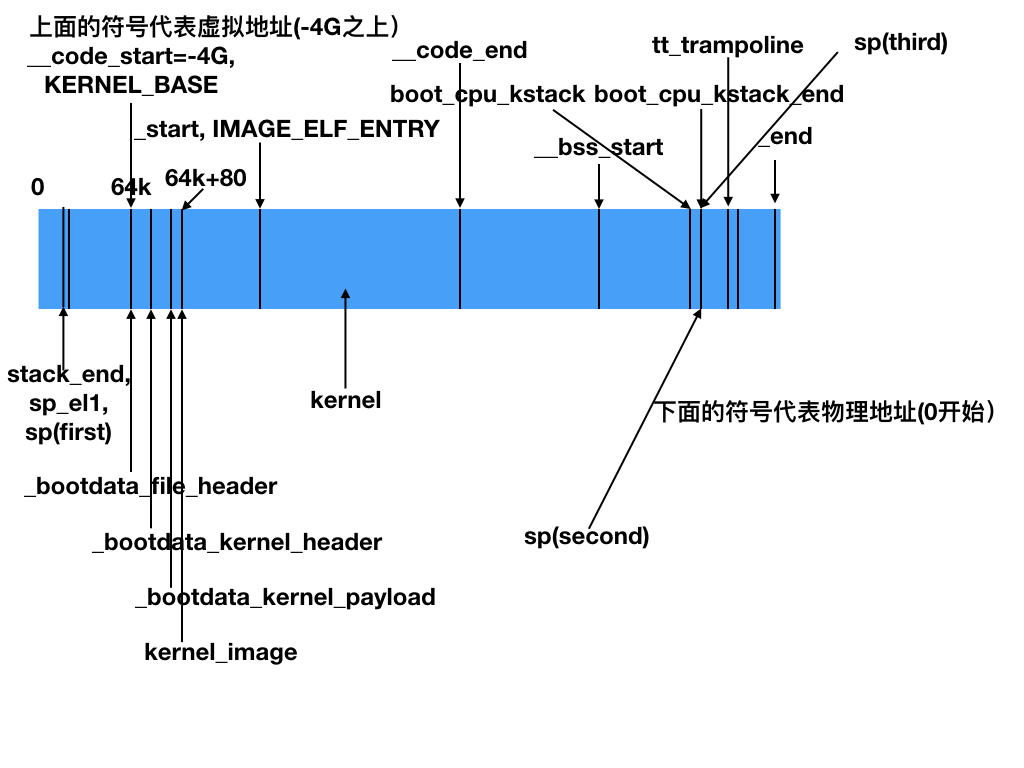
\includegraphics[scale=0.45]{zircon.png}

\subsection{副cpu}
\begin{enumerate}
    \item 切换到el1
    \item 等待主cpu把\verb!arm64_secondary_sp_list!设置好。在此之前
          会执行wfe。如果在主cpu设置之前执行的话,副cpu会进入死循环。
          但是主cpu会在bootstrap2里调用\verb!psci_smc_call!重启副cpu。实际调用的是smc 0.
          smc的异常处理配置是firmware设置的。在Zircon的代码中没有对
          \verb|vbar_el3|的设置。一个例子:在u-boot,armv8/psci.S里有对\verb|vbar_el3|
          的设置。但是很有可能应该是arm trusted firmware设置的这个。
    \item 最后进入\verb!arm64_secondary_entry()!
\end{enumerate}

